\documentclass[a4paper]{article}
\usepackage[a4paper,margin=1in,landscape]{geometry}
\usepackage[utf8]{inputenc}
\usepackage[T1]{fontenc}
\usepackage{longtable}
\usepackage[table,svgnames]{xcolor}
\usepackage{colortbl}
\usepackage{pgfplots}
\pgfplotsset{width=10cm,compat=1.14}
\usepgfplotslibrary{dateplot}
\usetikzlibrary{plotmarks}
\usepackage{booktabs}
\usepackage{array}
\usepackage{eurosym}
\usepackage{forest}
\usepackage{listings}
\usepackage{multicol}
\usepackage{fancyhdr}
\pagestyle{fancy}
\lfoot{Section \leftmark}
\cfoot{}
\rfoot{\thepage}
\rhead{Generated: \today}
\chead{}
\lhead{Publication Report}
\usepackage{hyperref}
\title{Publication Report}
\author{H. Simonis}
\date{Report Generated on \today}

\begin{document}
\maketitle
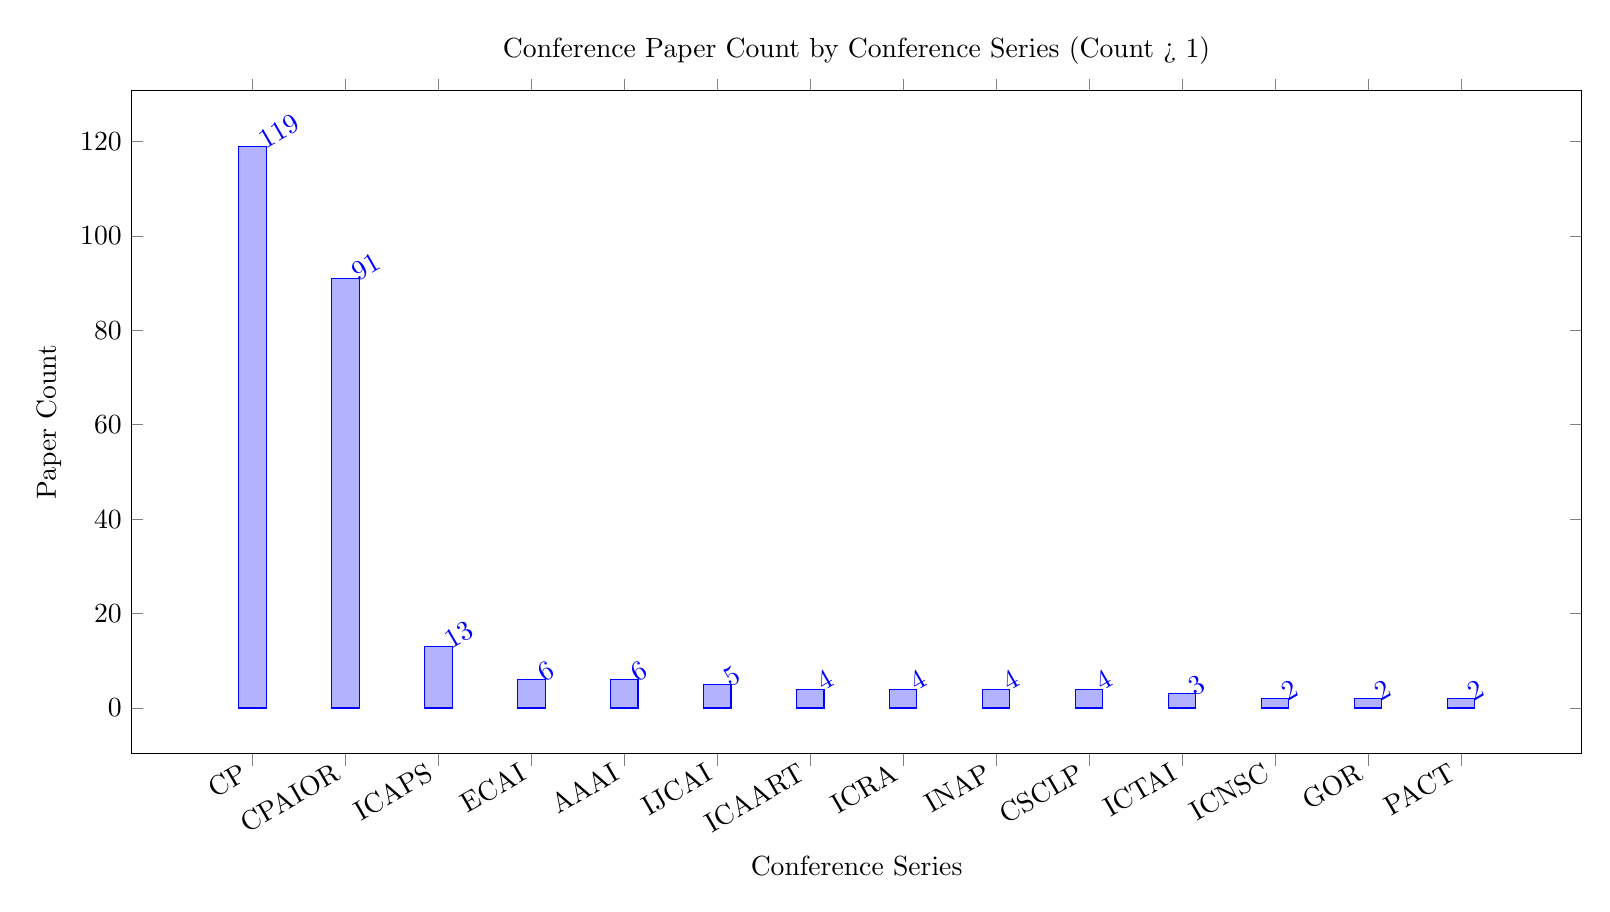
\begin{tikzpicture}
\begin{axis}[title=Conference Paper Count by Conference Series (Count > 1),xlabel=Conference Series,ylabel=Paper Count,
width=20cm,height=10cm,ybar,
symbolic x coords={CP,CPAIOR,ICAPS,ECAI,AAAI,IJCAI,ICAART,ICRA,INAP,CSCLP,ICTAI,ICNSC,GOR,PACT},
    xtick=data,nodes near coords, nodes near coords align={rotate=30),anchor=west},x tick label style={rotate=30),anchor=east}]
\addplot+[] coordinates {
(CP,119.000000)
(CPAIOR,91.000000)
(ICAPS,13.000000)
(ECAI,6.000000)
(AAAI,6.000000)
(IJCAI,5.000000)
(ICAART,4.000000)
(ICRA,4.000000)
(INAP,4.000000)
(CSCLP,4.000000)
(ICTAI,3.000000)
(ICNSC,2.000000)
(GOR,2.000000)
(PACT,2.000000)
};
\end{axis}
\end{tikzpicture}

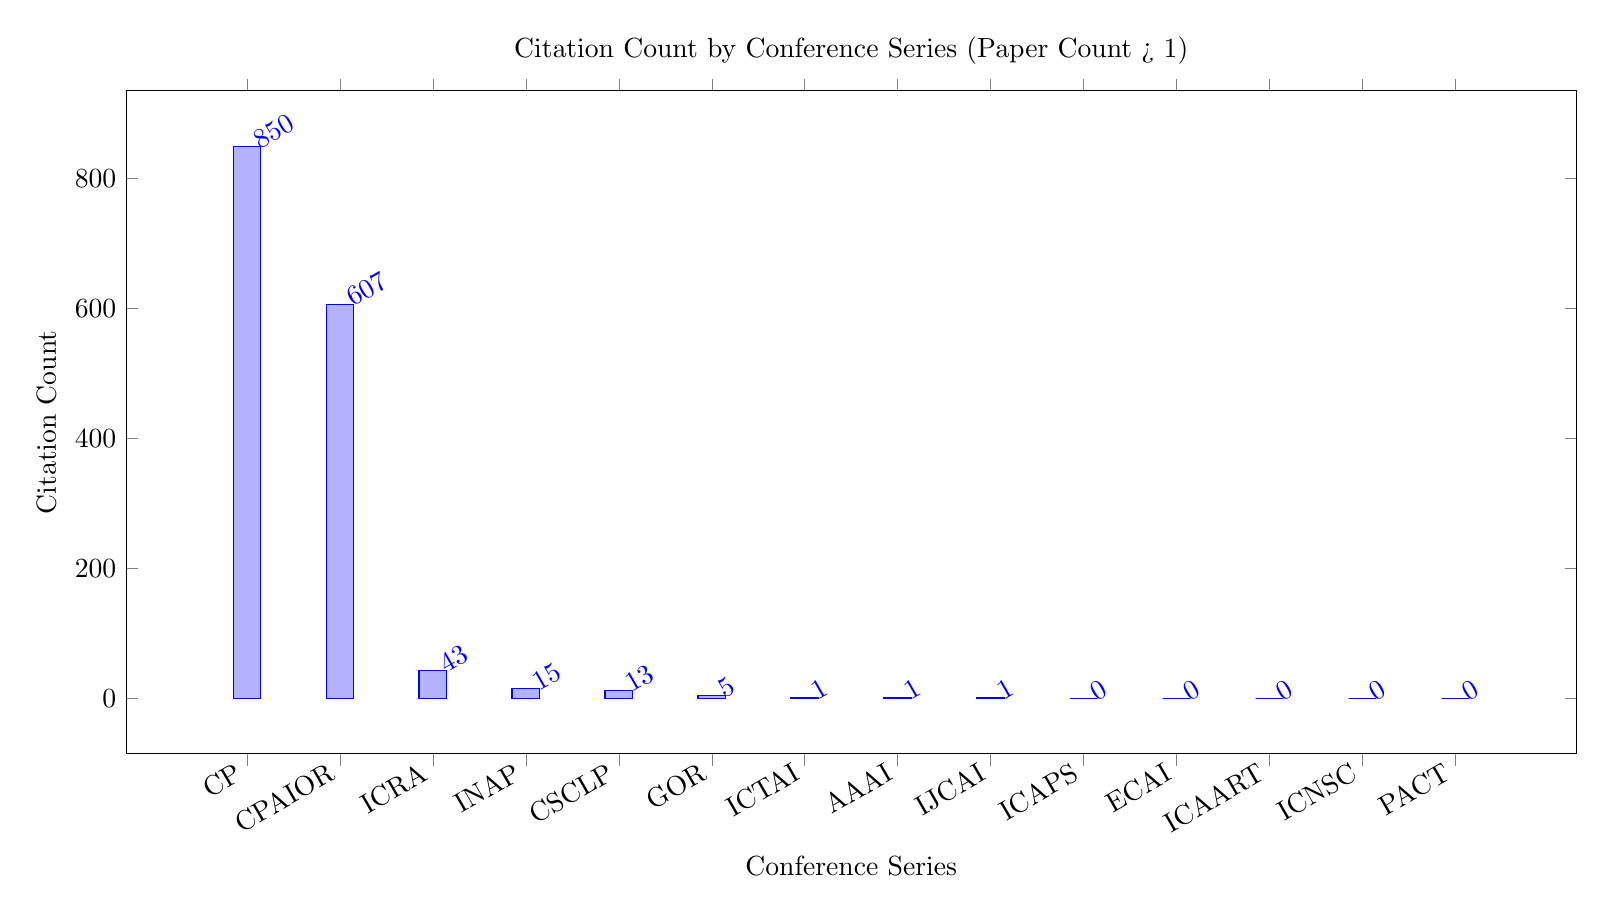
\begin{tikzpicture}
\begin{axis}[title=Citation Count by Conference Series (Paper Count > 1),xlabel=Conference Series,ylabel=Citation Count,
width=20cm,height=10cm,ybar,
symbolic x coords={CP,CPAIOR,ICRA,INAP,CSCLP,GOR,ICTAI,AAAI,IJCAI,ICAPS,ECAI,ICAART,ICNSC,PACT},
    xtick=data,nodes near coords, nodes near coords align={rotate=30),anchor=west},x tick label style={rotate=30),anchor=east}]
\addplot+[] coordinates {
(CP,850.000000)
(CPAIOR,607.000000)
(ICRA,43.000000)
(INAP,15.000000)
(CSCLP,13.000000)
(GOR,5.000000)
(ICTAI,1.000000)
(AAAI,1.000000)
(IJCAI,1.000000)
(ICAPS,0.000000)
(ECAI,0.000000)
(ICAART,0.000000)
(ICNSC,0.000000)
(PACT,0.000000)
};
\end{axis}
\end{tikzpicture}

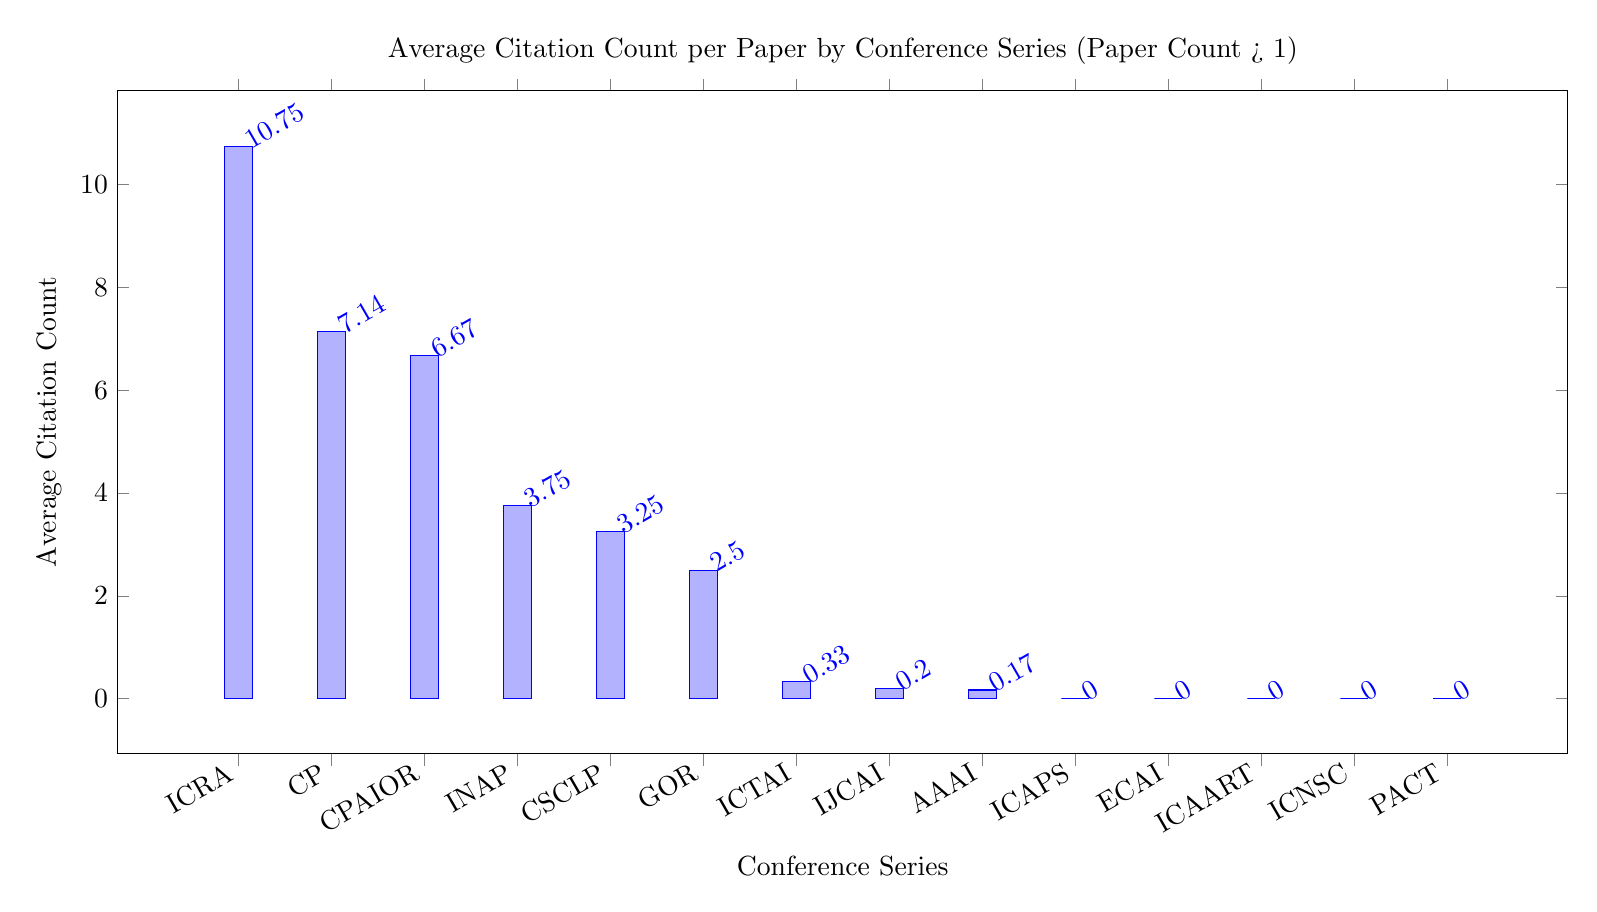
\begin{tikzpicture}
\begin{axis}[title=Average Citation Count per Paper by Conference Series (Paper Count > 1),xlabel=Conference Series,ylabel=Average Citation Count,
width=20cm,height=10cm,ybar,
symbolic x coords={ICRA,CP,CPAIOR,INAP,CSCLP,GOR,ICTAI,IJCAI,AAAI,ICAPS,ECAI,ICAART,ICNSC,PACT},
    xtick=data,nodes near coords, nodes near coords align={rotate=30),anchor=west},x tick label style={rotate=30),anchor=east}]
\addplot+[] coordinates {
(ICRA,10.750000)
(CP,7.142857)
(CPAIOR,6.670330)
(INAP,3.750000)
(CSCLP,3.250000)
(GOR,2.500000)
(ICTAI,0.333333)
(IJCAI,0.200000)
(AAAI,0.166667)
(ICAPS,0.000000)
(ECAI,0.000000)
(ICAART,0.000000)
(ICNSC,0.000000)
(PACT,0.000000)
};
\end{axis}
\end{tikzpicture}

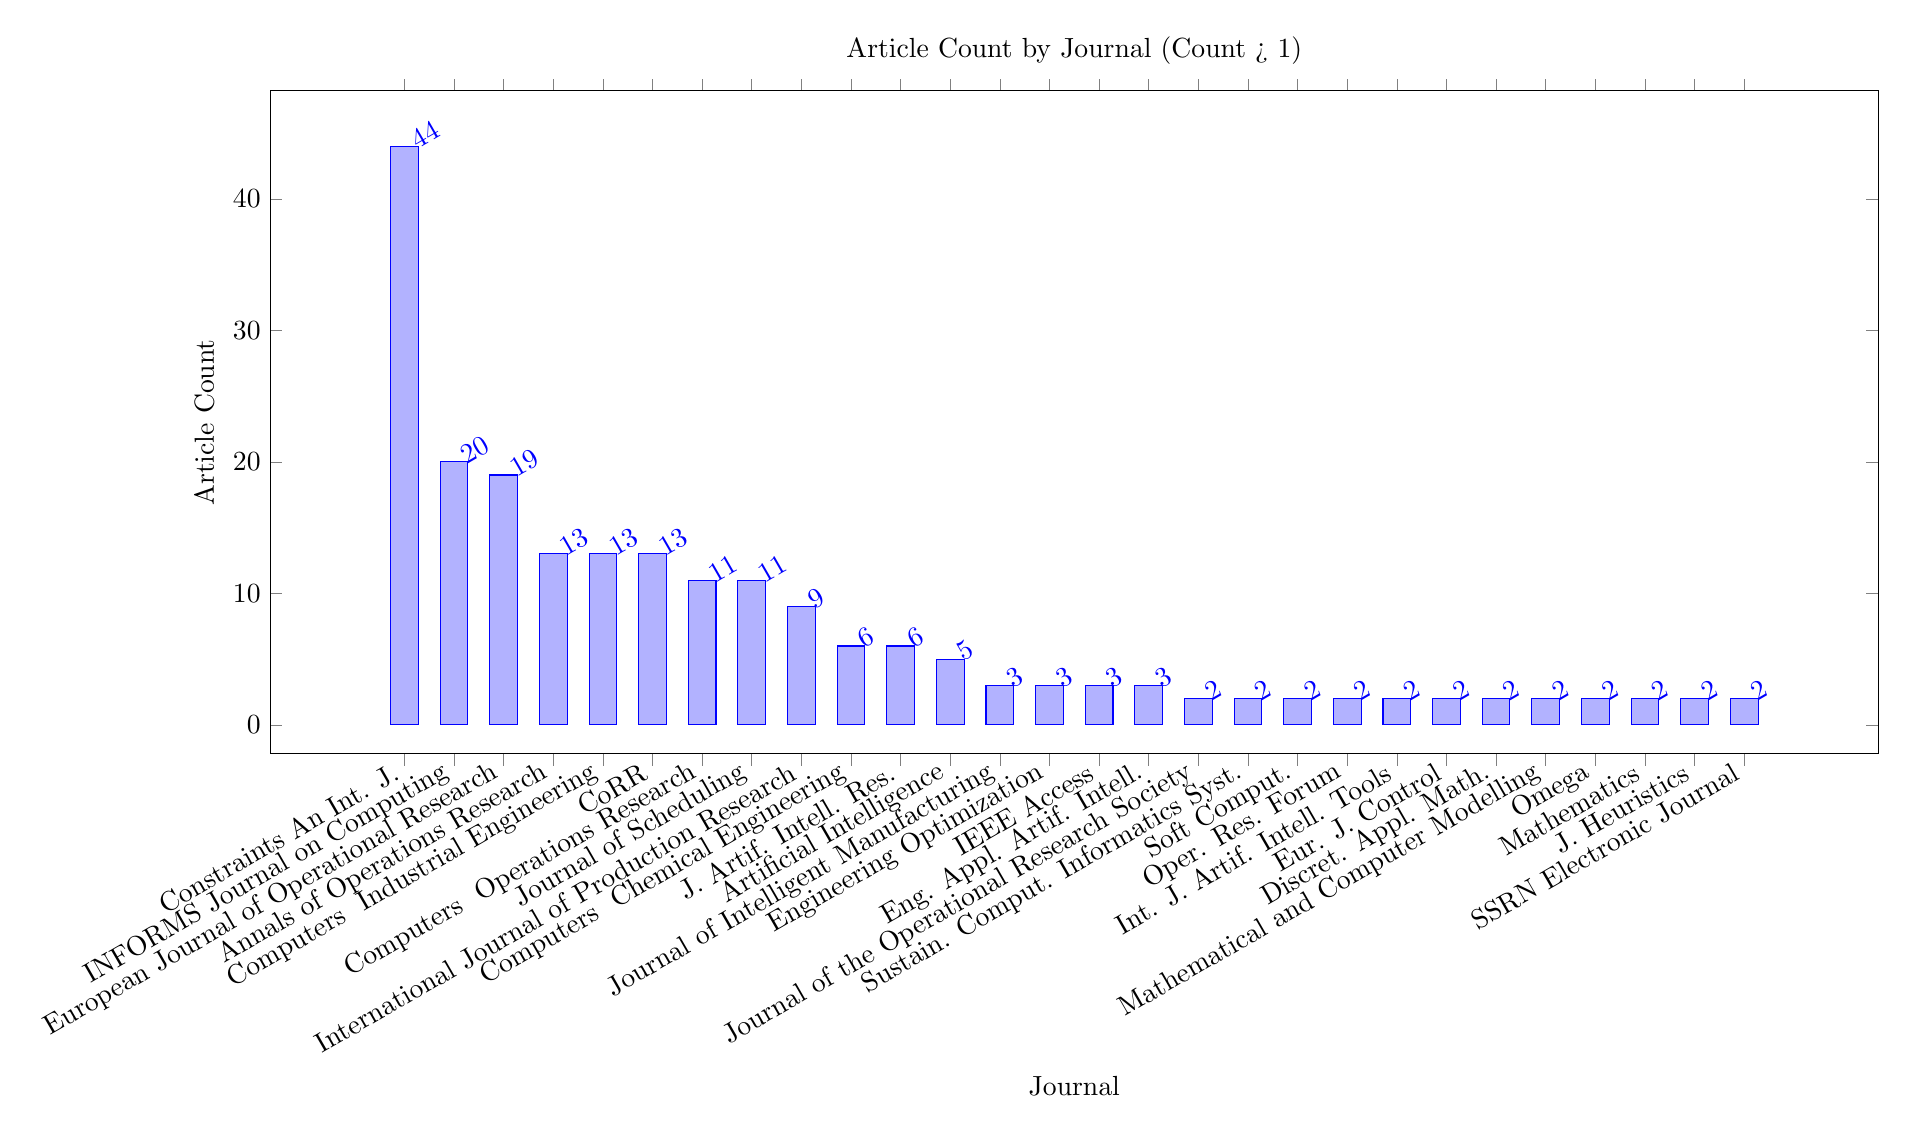
\begin{tikzpicture}
\begin{axis}[title=Article Count by Journal (Count > 1),xlabel=Journal,ylabel=Article Count,
width=22cm,height=10cm,ybar,
symbolic x coords={Constraints An Int. J.,INFORMS Journal on Computing,European Journal of Operational Research,Annals of Operations Research,Computers \  Industrial Engineering,CoRR,Computers \  Operations Research,Journal of Scheduling,International Journal of Production Research,Computers \  Chemical Engineering,J. Artif. Intell. Res.,Artificial Intelligence,Journal of Intelligent Manufacturing,Engineering Optimization,{IEEE} Access,Eng. Appl. Artif. Intell.,Journal of the Operational Research Society,Sustain. Comput. Informatics Syst.,Soft Comput.,Oper. Res. Forum,Int. J. Artif. Intell. Tools,Eur. J. Control,Discret. Appl. Math.,Mathematical and Computer Modelling,Omega,Mathematics,J. Heuristics,SSRN Electronic Journal},
    xtick=data,nodes near coords, nodes near coords align={rotate=30),anchor=west},x tick label style={rotate=30),anchor=east}]
\addplot+[] coordinates {
(Constraints An Int. J.,44.000000)
(INFORMS Journal on Computing,20.000000)
(European Journal of Operational Research,19.000000)
(Annals of Operations Research,13.000000)
(Computers \  Industrial Engineering,13.000000)
(CoRR,13.000000)
(Computers \  Operations Research,11.000000)
(Journal of Scheduling,11.000000)
(International Journal of Production Research,9.000000)
(Computers \  Chemical Engineering,6.000000)
(J. Artif. Intell. Res.,6.000000)
(Artificial Intelligence,5.000000)
(Journal of Intelligent Manufacturing,3.000000)
(Engineering Optimization,3.000000)
({IEEE} Access,3.000000)
(Eng. Appl. Artif. Intell.,3.000000)
(Journal of the Operational Research Society,2.000000)
(Sustain. Comput. Informatics Syst.,2.000000)
(Soft Comput.,2.000000)
(Oper. Res. Forum,2.000000)
(Int. J. Artif. Intell. Tools,2.000000)
(Eur. J. Control,2.000000)
(Discret. Appl. Math.,2.000000)
(Mathematical and Computer Modelling,2.000000)
(Omega,2.000000)
(Mathematics,2.000000)
(J. Heuristics,2.000000)
(SSRN Electronic Journal,2.000000)
};
\end{axis}
\end{tikzpicture}

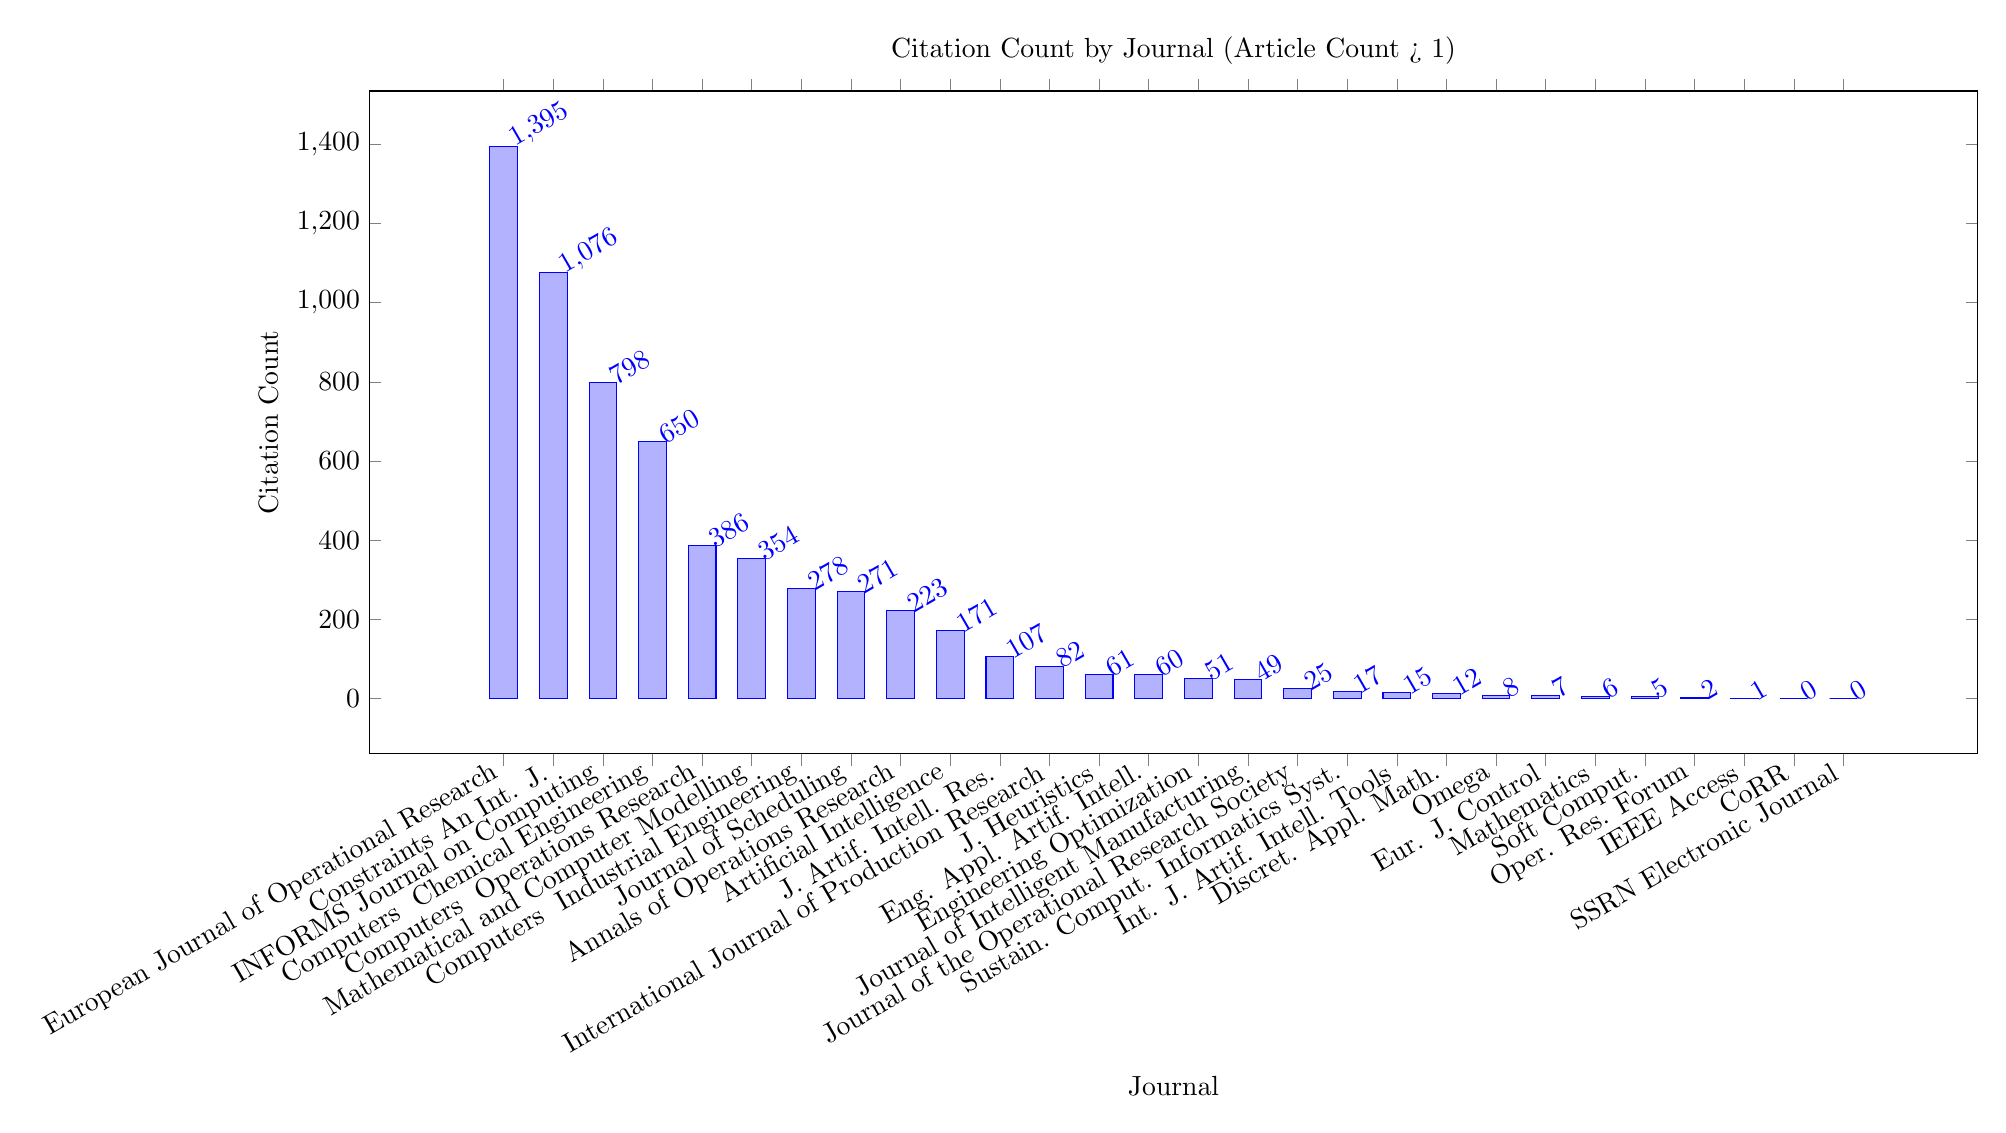
\begin{tikzpicture}
\begin{axis}[title=Citation Count by Journal (Article Count > 1),xlabel=Journal,ylabel=Citation Count,
width=22cm,height=10cm,ybar,
symbolic x coords={European Journal of Operational Research,Constraints An Int. J.,INFORMS Journal on Computing,Computers \  Chemical Engineering,Computers \  Operations Research,Mathematical and Computer Modelling,Computers \  Industrial Engineering,Journal of Scheduling,Annals of Operations Research,Artificial Intelligence,J. Artif. Intell. Res.,International Journal of Production Research,J. Heuristics,Eng. Appl. Artif. Intell.,Engineering Optimization,Journal of Intelligent Manufacturing,Journal of the Operational Research Society,Sustain. Comput. Informatics Syst.,Int. J. Artif. Intell. Tools,Discret. Appl. Math.,Omega,Eur. J. Control,Mathematics,Soft Comput.,Oper. Res. Forum,{IEEE} Access,CoRR,SSRN Electronic Journal},
    xtick=data,nodes near coords, nodes near coords align={rotate=30),anchor=west},x tick label style={rotate=30),anchor=east}]
\addplot+[] coordinates {
(European Journal of Operational Research,1395.000000)
(Constraints An Int. J.,1076.000000)
(INFORMS Journal on Computing,798.000000)
(Computers \  Chemical Engineering,650.000000)
(Computers \  Operations Research,386.000000)
(Mathematical and Computer Modelling,354.000000)
(Computers \  Industrial Engineering,278.000000)
(Journal of Scheduling,271.000000)
(Annals of Operations Research,223.000000)
(Artificial Intelligence,171.000000)
(J. Artif. Intell. Res.,107.000000)
(International Journal of Production Research,82.000000)
(J. Heuristics,61.000000)
(Eng. Appl. Artif. Intell.,60.000000)
(Engineering Optimization,51.000000)
(Journal of Intelligent Manufacturing,49.000000)
(Journal of the Operational Research Society,25.000000)
(Sustain. Comput. Informatics Syst.,17.000000)
(Int. J. Artif. Intell. Tools,15.000000)
(Discret. Appl. Math.,12.000000)
(Omega,8.000000)
(Eur. J. Control,7.000000)
(Mathematics,6.000000)
(Soft Comput.,5.000000)
(Oper. Res. Forum,2.000000)
({IEEE} Access,1.000000)
(CoRR,0.000000)
(SSRN Electronic Journal,0.000000)
};
\end{axis}
\end{tikzpicture}

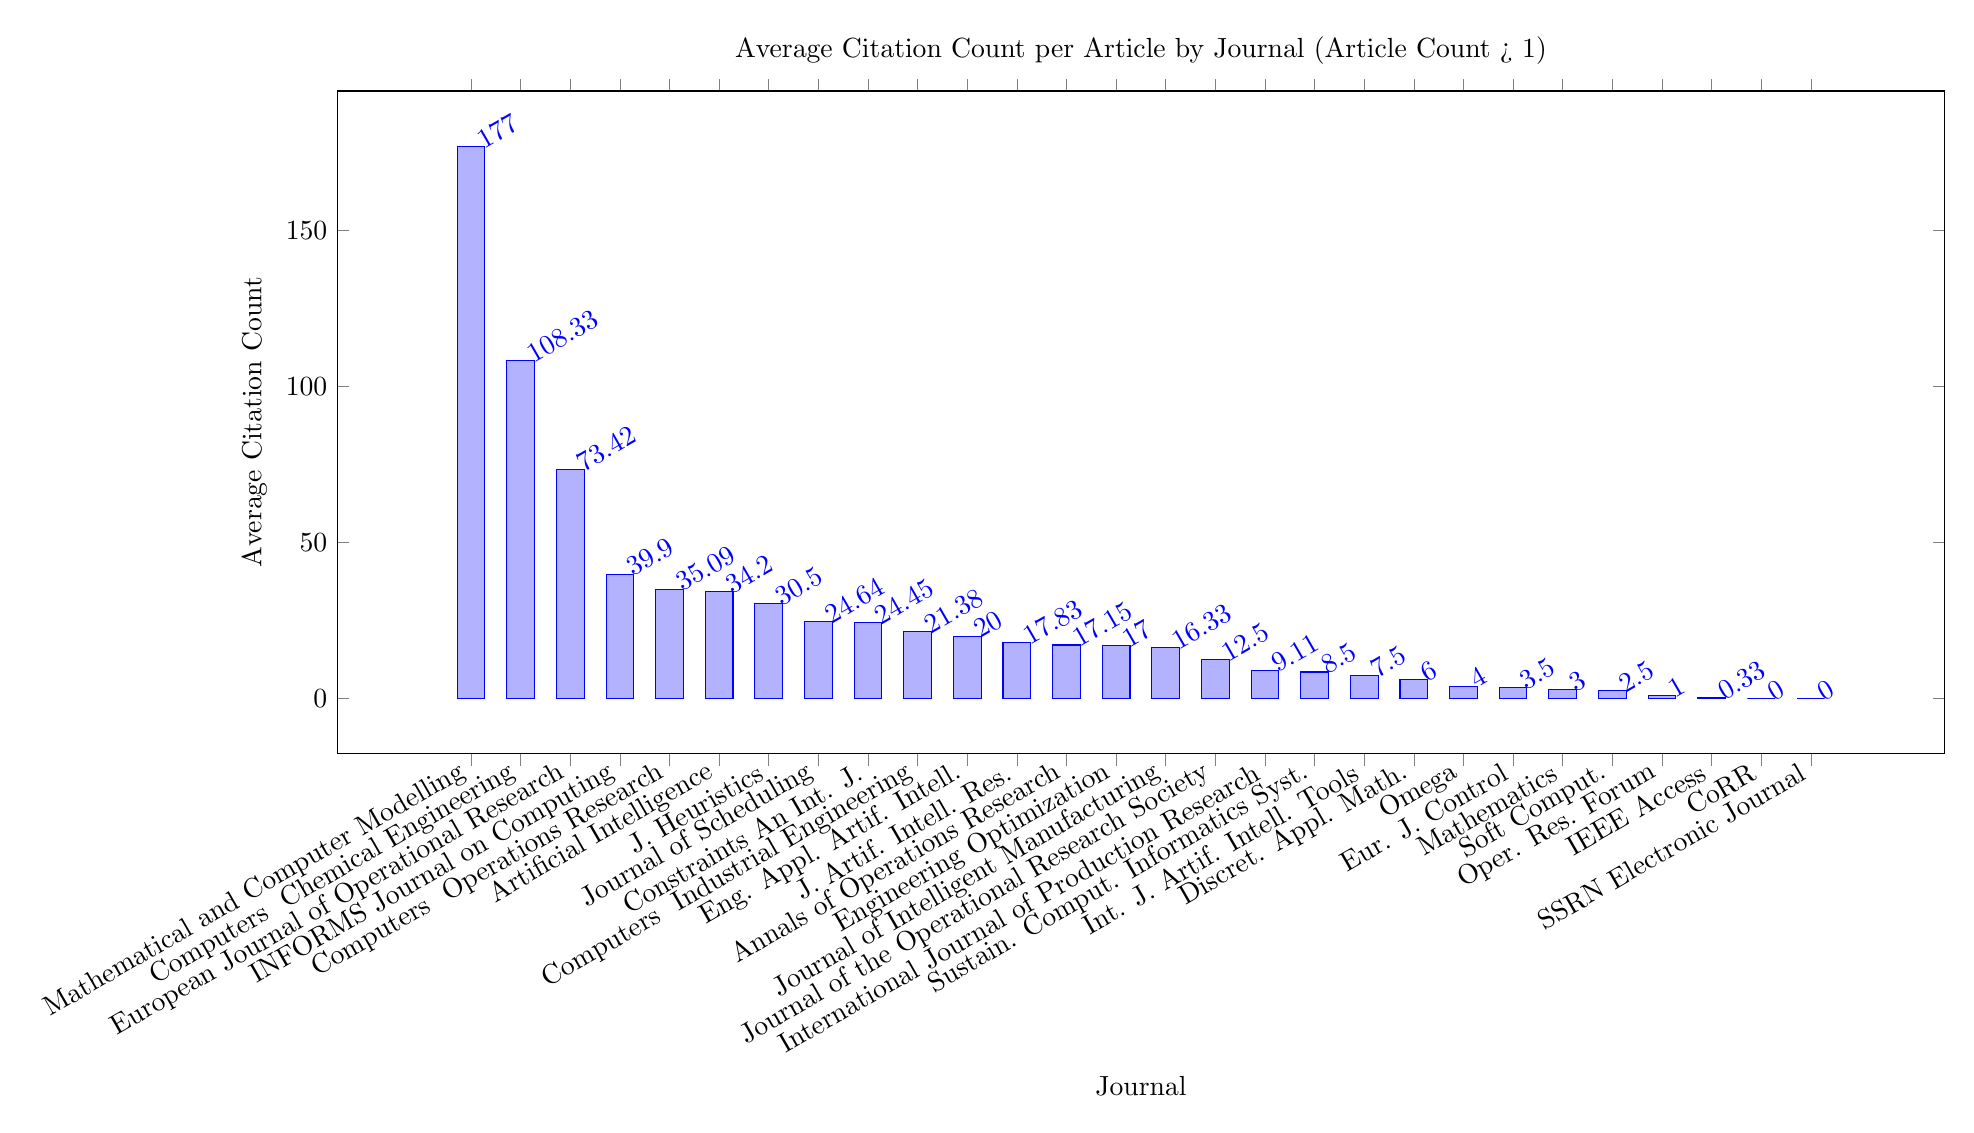
\begin{tikzpicture}
\begin{axis}[title=Average Citation Count per Article by Journal (Article Count > 1),xlabel=Journal,ylabel=Average Citation Count,
width=22cm,height=10cm,ybar,
symbolic x coords={Mathematical and Computer Modelling,Computers \  Chemical Engineering,European Journal of Operational Research,INFORMS Journal on Computing,Computers \  Operations Research,Artificial Intelligence,J. Heuristics,Journal of Scheduling,Constraints An Int. J.,Computers \  Industrial Engineering,Eng. Appl. Artif. Intell.,J. Artif. Intell. Res.,Annals of Operations Research,Engineering Optimization,Journal of Intelligent Manufacturing,Journal of the Operational Research Society,International Journal of Production Research,Sustain. Comput. Informatics Syst.,Int. J. Artif. Intell. Tools,Discret. Appl. Math.,Omega,Eur. J. Control,Mathematics,Soft Comput.,Oper. Res. Forum,{IEEE} Access,CoRR,SSRN Electronic Journal},
    xtick=data,nodes near coords, nodes near coords align={rotate=30),anchor=west},x tick label style={rotate=30),anchor=east}]
\addplot+[] coordinates {
(Mathematical and Computer Modelling,177.000000)
(Computers \  Chemical Engineering,108.333333)
(European Journal of Operational Research,73.421053)
(INFORMS Journal on Computing,39.900000)
(Computers \  Operations Research,35.090909)
(Artificial Intelligence,34.200000)
(J. Heuristics,30.500000)
(Journal of Scheduling,24.636364)
(Constraints An Int. J.,24.454545)
(Computers \  Industrial Engineering,21.384615)
(Eng. Appl. Artif. Intell.,20.000000)
(J. Artif. Intell. Res.,17.833333)
(Annals of Operations Research,17.153846)
(Engineering Optimization,17.000000)
(Journal of Intelligent Manufacturing,16.333333)
(Journal of the Operational Research Society,12.500000)
(International Journal of Production Research,9.111111)
(Sustain. Comput. Informatics Syst.,8.500000)
(Int. J. Artif. Intell. Tools,7.500000)
(Discret. Appl. Math.,6.000000)
(Omega,4.000000)
(Eur. J. Control,3.500000)
(Mathematics,3.000000)
(Soft Comput.,2.500000)
(Oper. Res. Forum,1.000000)
({IEEE} Access,0.333333)
(CoRR,0.000000)
(SSRN Electronic Journal,0.000000)
};
\end{axis}
\end{tikzpicture}

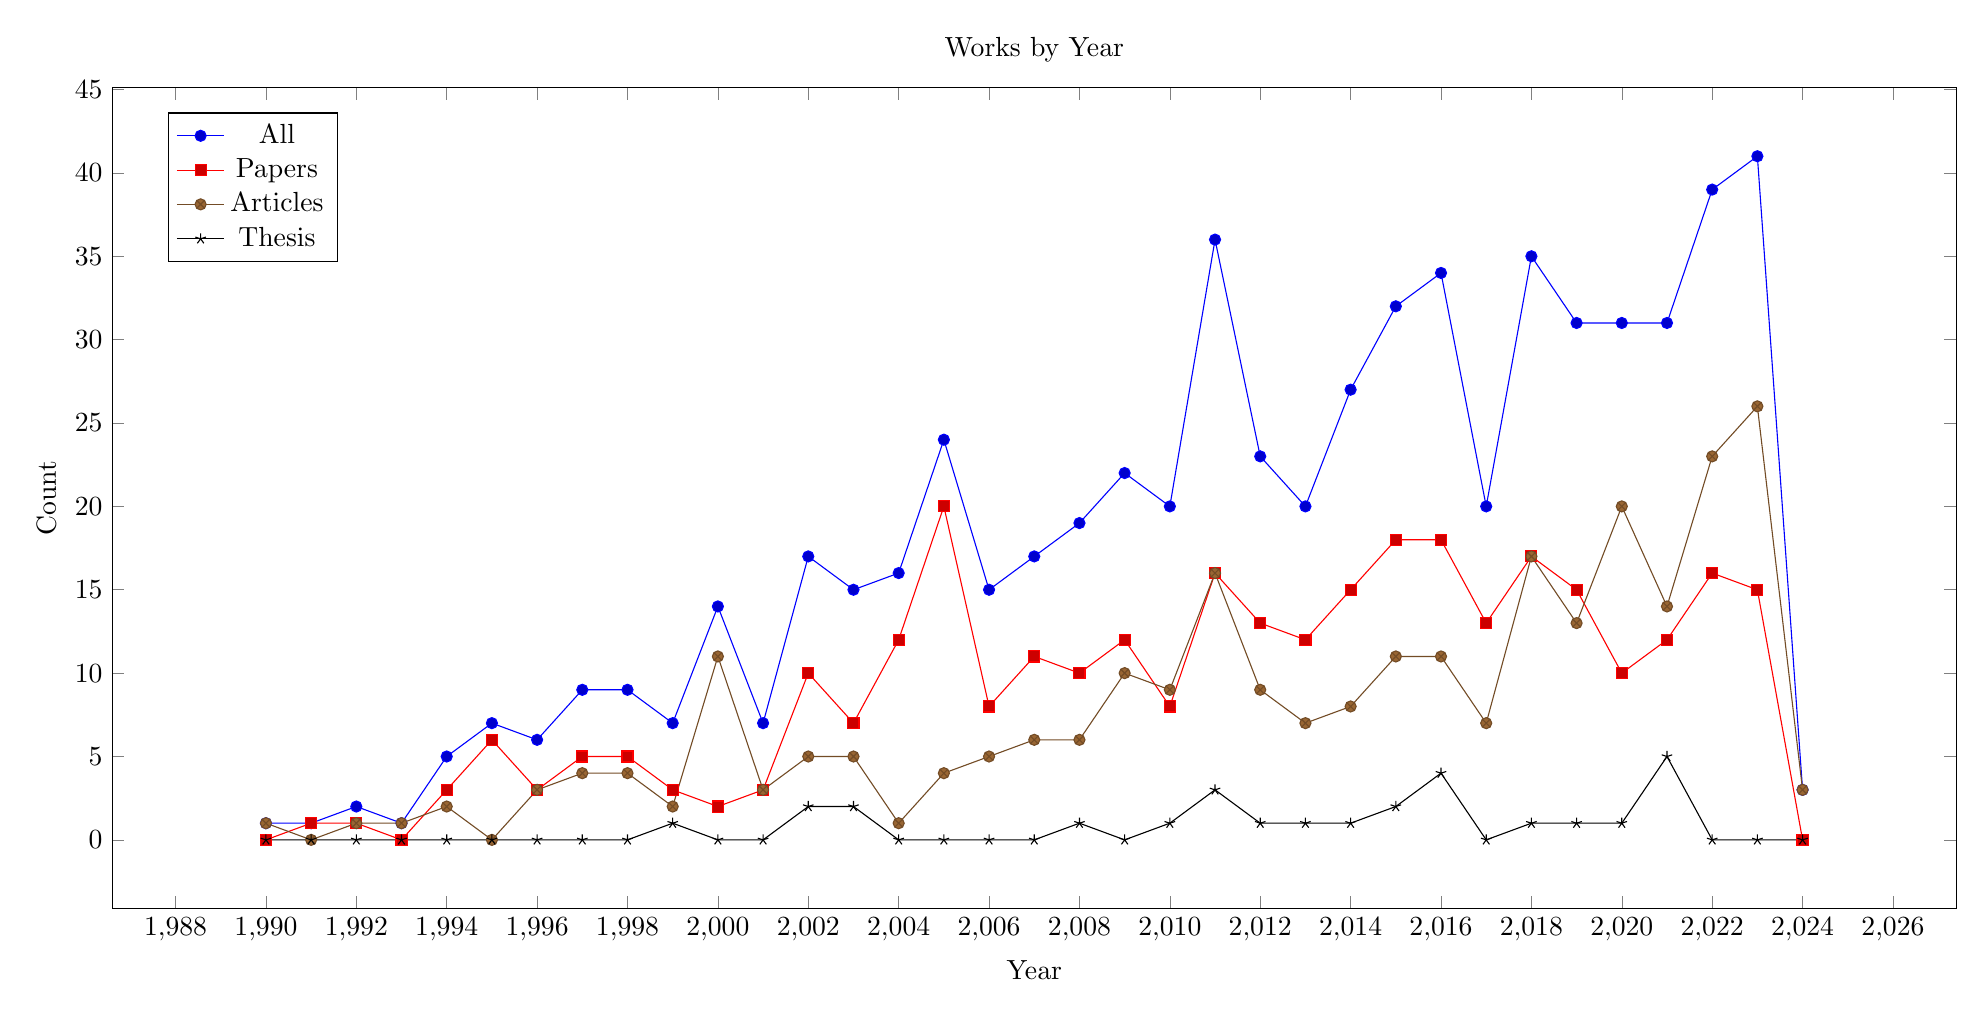
\begin{tikzpicture}
\begin{axis}[title=Works by Year,xlabel=Year,ylabel=Count,legend pos=north west,,width=25cm,height=12cm]
\addplot+[] coordinates {
    (1990.00,1.00000)
    (1991.00,1.00000)
    (1992.00,2.00000)
    (1993.00,1.00000)
    (1994.00,5.00000)
    (1995.00,7.00000)
    (1996.00,6.00000)
    (1997.00,9.00000)
    (1998.00,9.00000)
    (1999.00,7.00000)
    (2000.00,14.0000)
    (2001.00,7.00000)
    (2002.00,17.0000)
    (2003.00,15.0000)
    (2004.00,16.0000)
    (2005.00,24.0000)
    (2006.00,15.0000)
    (2007.00,17.0000)
    (2008.00,19.0000)
    (2009.00,22.0000)
    (2010.00,20.0000)
    (2011.00,36.0000)
    (2012.00,23.0000)
    (2013.00,20.0000)
    (2014.00,27.0000)
    (2015.00,32.0000)
    (2016.00,34.0000)
    (2017.00,20.0000)
    (2018.00,35.0000)
    (2019.00,31.0000)
    (2020.00,31.0000)
    (2021.00,31.0000)
    (2022.00,39.0000)
    (2023.00,41.0000)
    (2024.00,3.00000)
};
\addlegendentry{All}
\addplot+[] coordinates {
    (1990.00,0.00000)
    (1991.00,1.00000)
    (1992.00,1.00000)
    (1993.00,0.00000)
    (1994.00,3.00000)
    (1995.00,6.00000)
    (1996.00,3.00000)
    (1997.00,5.00000)
    (1998.00,5.00000)
    (1999.00,3.00000)
    (2000.00,2.00000)
    (2001.00,3.00000)
    (2002.00,10.0000)
    (2003.00,7.00000)
    (2004.00,12.0000)
    (2005.00,20.0000)
    (2006.00,8.00000)
    (2007.00,11.0000)
    (2008.00,10.0000)
    (2009.00,12.0000)
    (2010.00,8.00000)
    (2011.00,16.0000)
    (2012.00,13.0000)
    (2013.00,12.0000)
    (2014.00,15.0000)
    (2015.00,18.0000)
    (2016.00,18.0000)
    (2017.00,13.0000)
    (2018.00,17.0000)
    (2019.00,15.0000)
    (2020.00,10.0000)
    (2021.00,12.0000)
    (2022.00,16.0000)
    (2023.00,15.0000)
    (2024.00,0.00000)
};
\addlegendentry{Papers}
\addplot+[] coordinates {
    (1990.00,1.00000)
    (1991.00,0.00000)
    (1992.00,1.00000)
    (1993.00,1.00000)
    (1994.00,2.00000)
    (1995.00,0.00000)
    (1996.00,3.00000)
    (1997.00,4.00000)
    (1998.00,4.00000)
    (1999.00,2.00000)
    (2000.00,11.0000)
    (2001.00,3.00000)
    (2002.00,5.00000)
    (2003.00,5.00000)
    (2004.00,1.00000)
    (2005.00,4.00000)
    (2006.00,5.00000)
    (2007.00,6.00000)
    (2008.00,6.00000)
    (2009.00,10.0000)
    (2010.00,9.00000)
    (2011.00,16.0000)
    (2012.00,9.00000)
    (2013.00,7.00000)
    (2014.00,8.00000)
    (2015.00,11.0000)
    (2016.00,11.0000)
    (2017.00,7.00000)
    (2018.00,17.0000)
    (2019.00,13.0000)
    (2020.00,20.0000)
    (2021.00,14.0000)
    (2022.00,23.0000)
    (2023.00,26.0000)
    (2024.00,3.00000)
};
\addlegendentry{Articles}
\addplot+[] coordinates {
    (1990.00,0.00000)
    (1991.00,0.00000)
    (1992.00,0.00000)
    (1993.00,0.00000)
    (1994.00,0.00000)
    (1995.00,0.00000)
    (1996.00,0.00000)
    (1997.00,0.00000)
    (1998.00,0.00000)
    (1999.00,1.00000)
    (2000.00,0.00000)
    (2001.00,0.00000)
    (2002.00,2.00000)
    (2003.00,2.00000)
    (2004.00,0.00000)
    (2005.00,0.00000)
    (2006.00,0.00000)
    (2007.00,0.00000)
    (2008.00,1.00000)
    (2009.00,0.00000)
    (2010.00,1.00000)
    (2011.00,3.00000)
    (2012.00,1.00000)
    (2013.00,1.00000)
    (2014.00,1.00000)
    (2015.00,2.00000)
    (2016.00,4.00000)
    (2017.00,0.00000)
    (2018.00,1.00000)
    (2019.00,1.00000)
    (2020.00,1.00000)
    (2021.00,5.00000)
    (2022.00,0.00000)
    (2023.00,0.00000)
    (2024.00,0.00000)
};
\addlegendentry{Thesis}
\end{axis}
\end{tikzpicture}

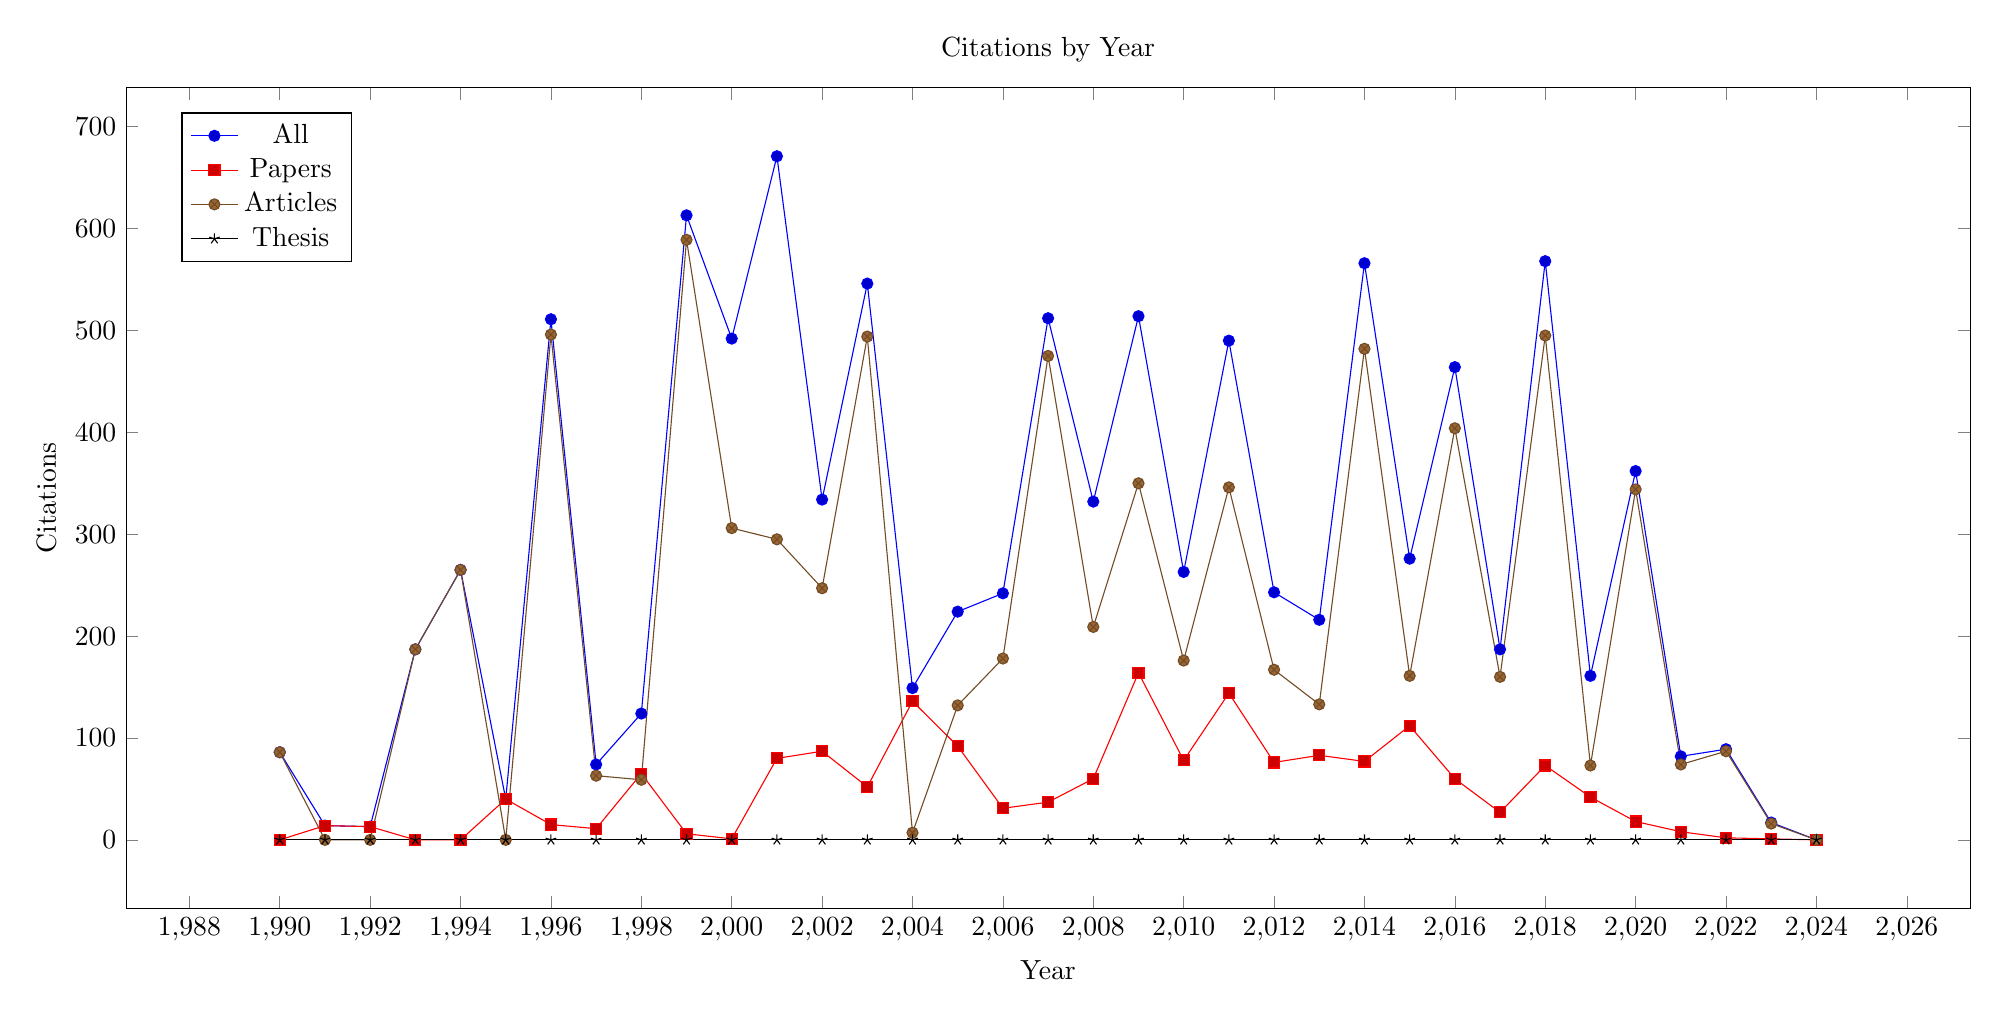
\begin{tikzpicture}
\begin{axis}[title=Citations by Year,xlabel=Year,ylabel=Citations,legend pos=north west,,width=25cm,height=12cm]
\addplot+[] coordinates {
    (1990.00,86.0000)
    (1991.00,14.0000)
    (1992.00,13.0000)
    (1993.00,187.000)
    (1994.00,265.000)
    (1995.00,40.0000)
    (1996.00,511.000)
    (1997.00,74.0000)
    (1998.00,124.000)
    (1999.00,613.000)
    (2000.00,492.000)
    (2001.00,671.000)
    (2002.00,334.000)
    (2003.00,546.000)
    (2004.00,149.000)
    (2005.00,224.000)
    (2006.00,242.000)
    (2007.00,512.000)
    (2008.00,332.000)
    (2009.00,514.000)
    (2010.00,263.000)
    (2011.00,490.000)
    (2012.00,243.000)
    (2013.00,216.000)
    (2014.00,566.000)
    (2015.00,276.000)
    (2016.00,464.000)
    (2017.00,187.000)
    (2018.00,568.000)
    (2019.00,161.000)
    (2020.00,362.000)
    (2021.00,82.0000)
    (2022.00,89.0000)
    (2023.00,17.0000)
    (2024.00,0.00000)
};
\addlegendentry{All}
\addplot+[] coordinates {
    (1990.00,0.00000)
    (1991.00,14.0000)
    (1992.00,13.0000)
    (1993.00,0.00000)
    (1994.00,0.00000)
    (1995.00,40.0000)
    (1996.00,15.0000)
    (1997.00,11.0000)
    (1998.00,65.0000)
    (1999.00,6.00000)
    (2000.00,1.00000)
    (2001.00,80.0000)
    (2002.00,87.0000)
    (2003.00,52.0000)
    (2004.00,136.000)
    (2005.00,92.0000)
    (2006.00,31.0000)
    (2007.00,37.0000)
    (2008.00,60.0000)
    (2009.00,164.000)
    (2010.00,78.0000)
    (2011.00,144.000)
    (2012.00,76.0000)
    (2013.00,83.0000)
    (2014.00,77.0000)
    (2015.00,112.000)
    (2016.00,60.0000)
    (2017.00,27.0000)
    (2018.00,73.0000)
    (2019.00,42.0000)
    (2020.00,18.0000)
    (2021.00,8.00000)
    (2022.00,2.00000)
    (2023.00,1.00000)
    (2024.00,0.00000)
};
\addlegendentry{Papers}
\addplot+[] coordinates {
    (1990.00,86.0000)
    (1991.00,0.00000)
    (1992.00,0.00000)
    (1993.00,187.000)
    (1994.00,265.000)
    (1995.00,0.00000)
    (1996.00,496.000)
    (1997.00,63.0000)
    (1998.00,59.0000)
    (1999.00,589.000)
    (2000.00,306.000)
    (2001.00,295.000)
    (2002.00,247.000)
    (2003.00,494.000)
    (2004.00,7.00000)
    (2005.00,132.000)
    (2006.00,178.000)
    (2007.00,475.000)
    (2008.00,209.000)
    (2009.00,350.000)
    (2010.00,176.000)
    (2011.00,346.000)
    (2012.00,167.000)
    (2013.00,133.000)
    (2014.00,482.000)
    (2015.00,161.000)
    (2016.00,404.000)
    (2017.00,160.000)
    (2018.00,495.000)
    (2019.00,73.0000)
    (2020.00,344.000)
    (2021.00,74.0000)
    (2022.00,87.0000)
    (2023.00,16.0000)
    (2024.00,0.00000)
};
\addlegendentry{Articles}
\addplot+[] coordinates {
    (1990.00,0.00000)
    (1991.00,0.00000)
    (1992.00,0.00000)
    (1993.00,0.00000)
    (1994.00,0.00000)
    (1995.00,0.00000)
    (1996.00,0.00000)
    (1997.00,0.00000)
    (1998.00,0.00000)
    (1999.00,0.00000)
    (2000.00,0.00000)
    (2001.00,0.00000)
    (2002.00,0.00000)
    (2003.00,0.00000)
    (2004.00,0.00000)
    (2005.00,0.00000)
    (2006.00,0.00000)
    (2007.00,0.00000)
    (2008.00,0.00000)
    (2009.00,0.00000)
    (2010.00,0.00000)
    (2011.00,0.00000)
    (2012.00,0.00000)
    (2013.00,0.00000)
    (2014.00,0.00000)
    (2015.00,0.00000)
    (2016.00,0.00000)
    (2017.00,0.00000)
    (2018.00,0.00000)
    (2019.00,0.00000)
    (2020.00,0.00000)
    (2021.00,0.00000)
    (2022.00,0.00000)
    (2023.00,0.00000)
    (2024.00,0.00000)
};
\addlegendentry{Thesis}
\end{axis}
\end{tikzpicture}

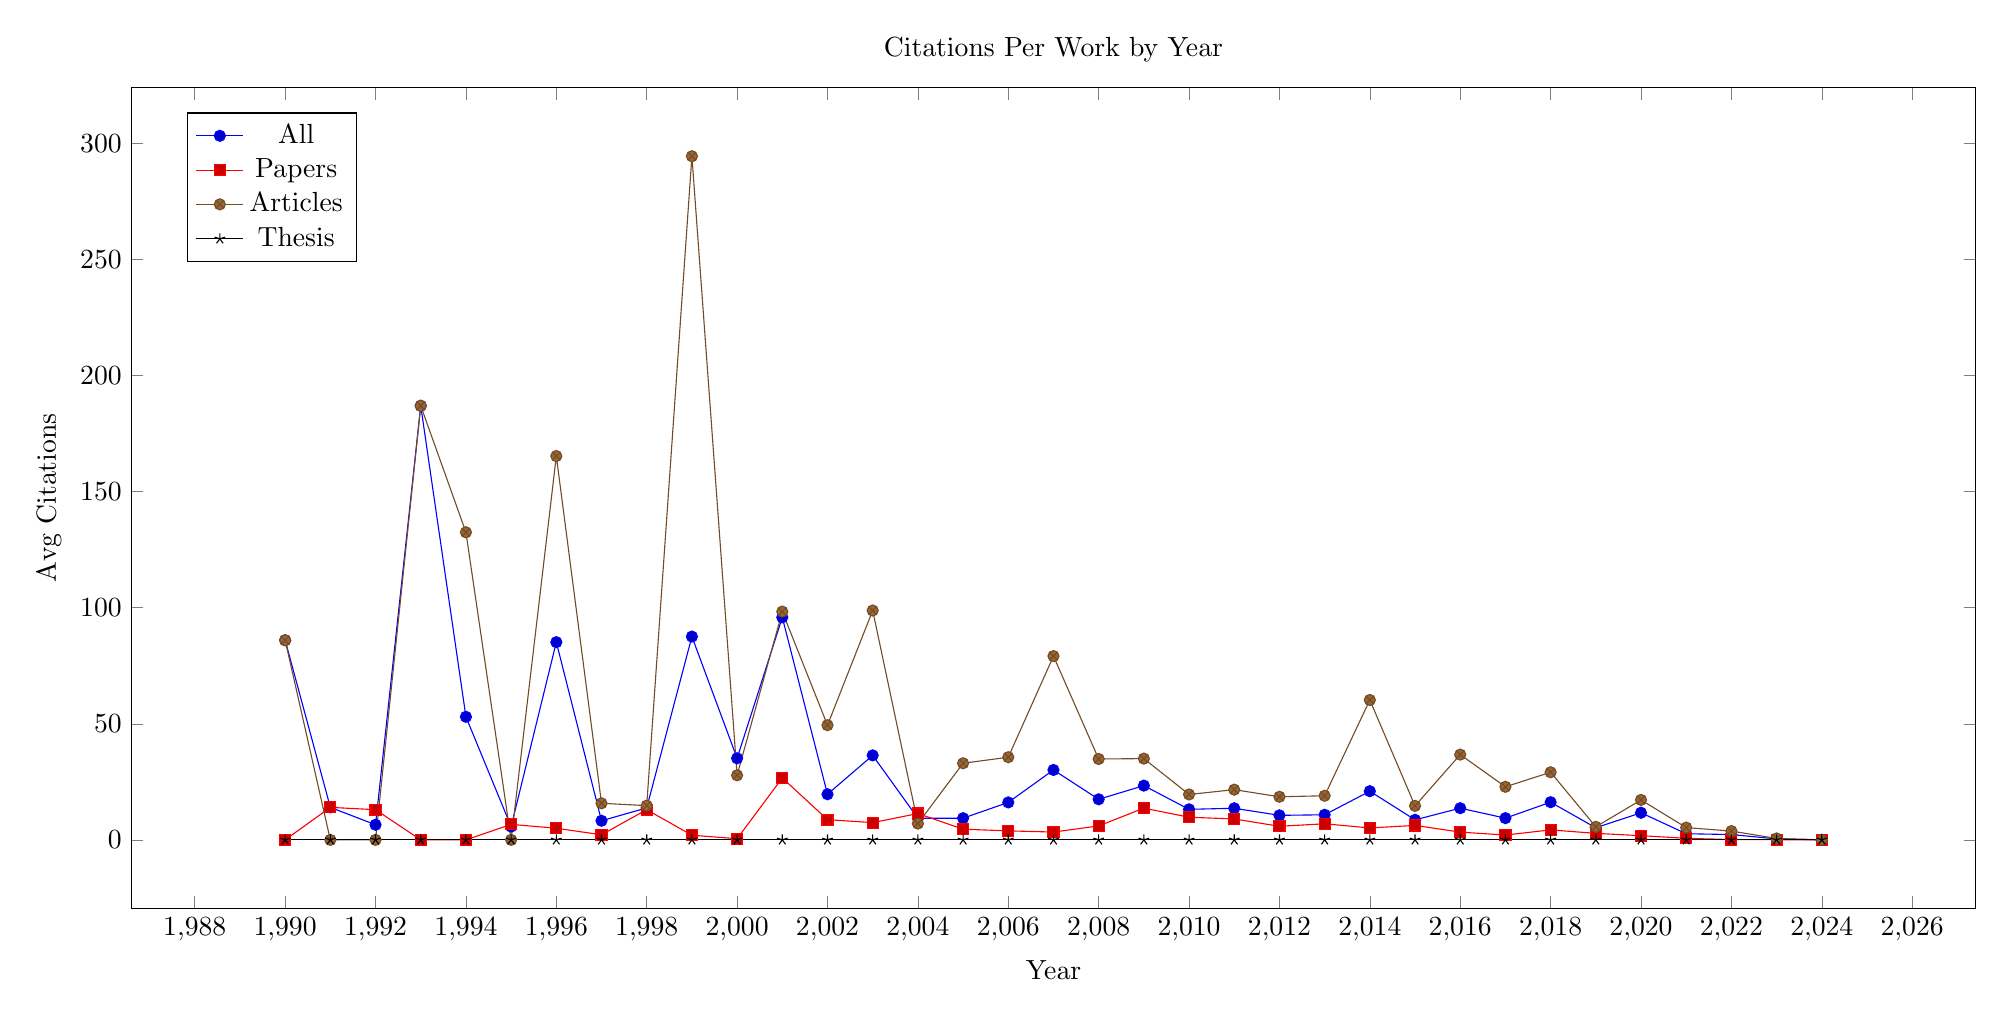
\begin{tikzpicture}
\begin{axis}[title=Citations Per Work by Year,xlabel=Year,ylabel=Avg Citations,legend pos=north west,,width=25cm,height=12cm]
\addplot+[] coordinates {
    (1990.00,86.0000)
    (1991.00,14.0000)
    (1992.00,6.50000)
    (1993.00,187.000)
    (1994.00,53.0000)
    (1995.00,5.71429)
    (1996.00,85.1667)
    (1997.00,8.22222)
    (1998.00,13.7778)
    (1999.00,87.5714)
    (2000.00,35.1429)
    (2001.00,95.8571)
    (2002.00,19.6471)
    (2003.00,36.4000)
    (2004.00,9.31250)
    (2005.00,9.33333)
    (2006.00,16.1333)
    (2007.00,30.1176)
    (2008.00,17.4737)
    (2009.00,23.3636)
    (2010.00,13.1500)
    (2011.00,13.6111)
    (2012.00,10.5652)
    (2013.00,10.8000)
    (2014.00,20.9630)
    (2015.00,8.62500)
    (2016.00,13.6471)
    (2017.00,9.35000)
    (2018.00,16.2286)
    (2019.00,5.19355)
    (2020.00,11.6774)
    (2021.00,2.64516)
    (2022.00,2.28205)
    (2023.00,0.414634)
    (2024.00,0.00000)
};
\addlegendentry{All}
\addplot+[] coordinates {
    (1990.00,0.00000)
    (1991.00,14.0000)
    (1992.00,13.0000)
    (1993.00,0.00000)
    (1994.00,0.00000)
    (1995.00,6.66667)
    (1996.00,5.00000)
    (1997.00,2.20000)
    (1998.00,13.0000)
    (1999.00,2.00000)
    (2000.00,0.500000)
    (2001.00,26.6667)
    (2002.00,8.70000)
    (2003.00,7.42857)
    (2004.00,11.3333)
    (2005.00,4.60000)
    (2006.00,3.87500)
    (2007.00,3.36364)
    (2008.00,6.00000)
    (2009.00,13.6667)
    (2010.00,9.75000)
    (2011.00,9.00000)
    (2012.00,5.84615)
    (2013.00,6.91667)
    (2014.00,5.13333)
    (2015.00,6.22222)
    (2016.00,3.33333)
    (2017.00,2.07692)
    (2018.00,4.29412)
    (2019.00,2.80000)
    (2020.00,1.80000)
    (2021.00,0.666667)
    (2022.00,0.125000)
    (2023.00,0.0666667)
    (2024.00,0.00000)
};
\addlegendentry{Papers}
\addplot+[] coordinates {
    (1990.00,86.0000)
    (1991.00,0.00000)
    (1992.00,0.00000)
    (1993.00,187.000)
    (1994.00,132.500)
    (1995.00,0.00000)
    (1996.00,165.333)
    (1997.00,15.7500)
    (1998.00,14.7500)
    (1999.00,294.500)
    (2000.00,27.8182)
    (2001.00,98.3333)
    (2002.00,49.4000)
    (2003.00,98.8000)
    (2004.00,7.00000)
    (2005.00,33.0000)
    (2006.00,35.6000)
    (2007.00,79.1667)
    (2008.00,34.8333)
    (2009.00,35.0000)
    (2010.00,19.5556)
    (2011.00,21.6250)
    (2012.00,18.5556)
    (2013.00,19.0000)
    (2014.00,60.2500)
    (2015.00,14.6364)
    (2016.00,36.7273)
    (2017.00,22.8571)
    (2018.00,29.1176)
    (2019.00,5.61538)
    (2020.00,17.2000)
    (2021.00,5.28571)
    (2022.00,3.78261)
    (2023.00,0.615385)
    (2024.00,0.00000)
};
\addlegendentry{Articles}
\addplot+[] coordinates {
    (1990.00,0.00000)
    (1991.00,0.00000)
    (1992.00,0.00000)
    (1993.00,0.00000)
    (1994.00,0.00000)
    (1995.00,0.00000)
    (1996.00,0.00000)
    (1997.00,0.00000)
    (1998.00,0.00000)
    (1999.00,0.00000)
    (2000.00,0.00000)
    (2001.00,0.00000)
    (2002.00,0.00000)
    (2003.00,0.00000)
    (2004.00,0.00000)
    (2005.00,0.00000)
    (2006.00,0.00000)
    (2007.00,0.00000)
    (2008.00,0.00000)
    (2009.00,0.00000)
    (2010.00,0.00000)
    (2011.00,0.00000)
    (2012.00,0.00000)
    (2013.00,0.00000)
    (2014.00,0.00000)
    (2015.00,0.00000)
    (2016.00,0.00000)
    (2017.00,0.00000)
    (2018.00,0.00000)
    (2019.00,0.00000)
    (2020.00,0.00000)
    (2021.00,0.00000)
    (2022.00,0.00000)
    (2023.00,0.00000)
    (2024.00,0.00000)
};
\addlegendentry{Thesis}
\end{axis}
\end{tikzpicture}

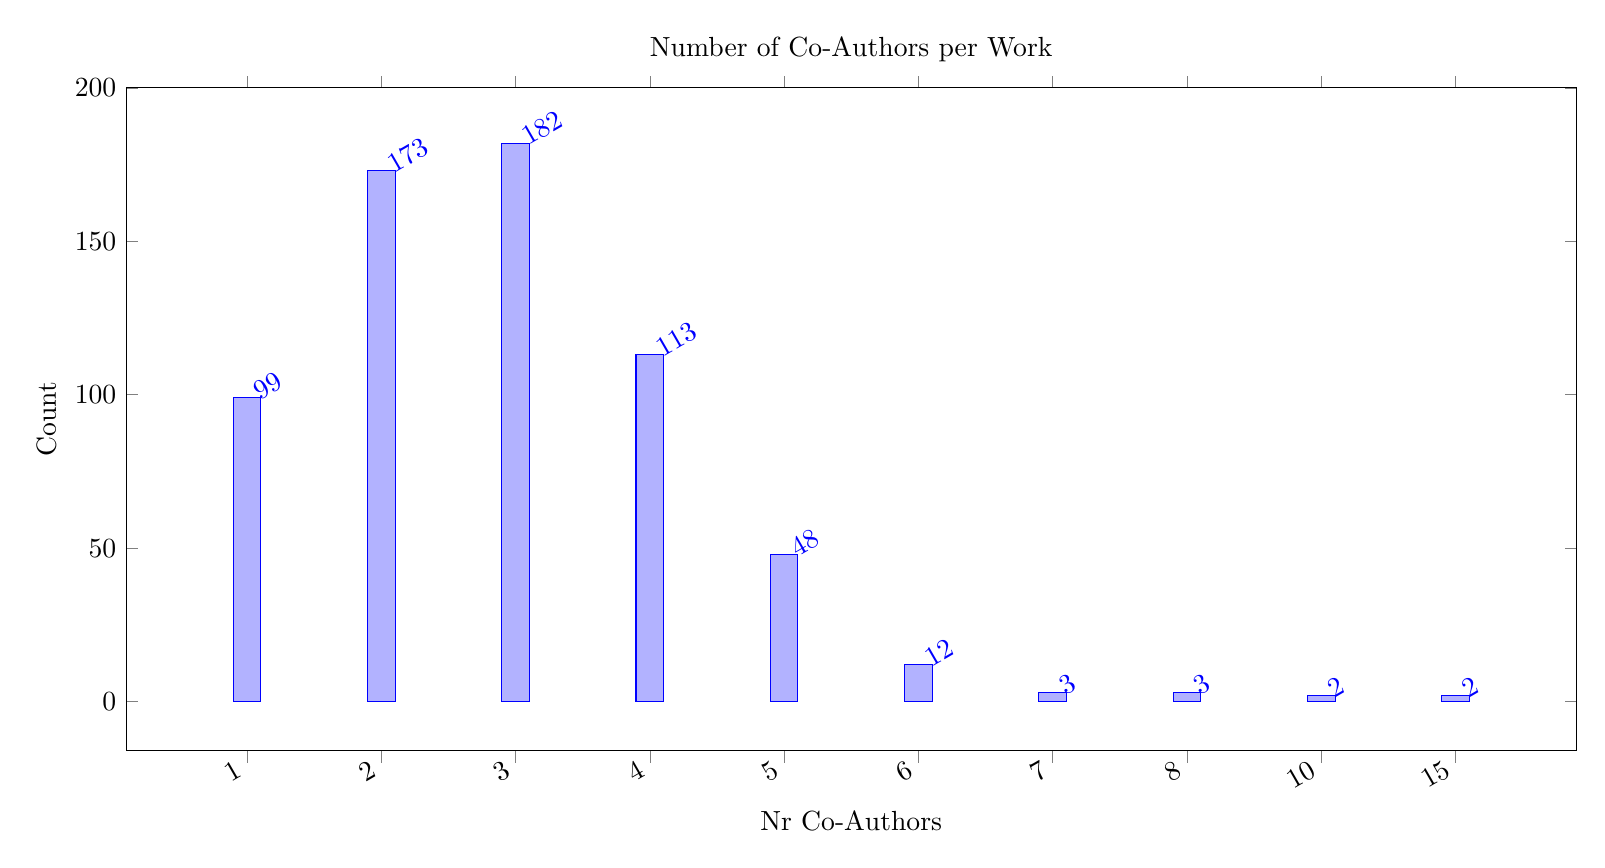
\begin{tikzpicture}
\begin{axis}[title=Number of Co-Authors per Work,xlabel=Nr Co-Authors,ylabel=Count,width=20cm,height=10cm,ybar,symbolic x coords={1,2,3,4,5,6,7,8,10,15},
    xtick=data,
    nodes near coords, 
    nodes near coords align={rotate=30,anchor=west},
    x tick label style={rotate=30,anchor=east},
]
\addplot+[] coordinates {
(1,99.000000)
(2,173.000000)
(3,182.000000)
(4,113.000000)
(5,48.000000)
(6,12.000000)
(7,3.000000)
(8,3.000000)
(10,2.000000)
(15,2.000000)
};
\end{axis}
\end{tikzpicture}

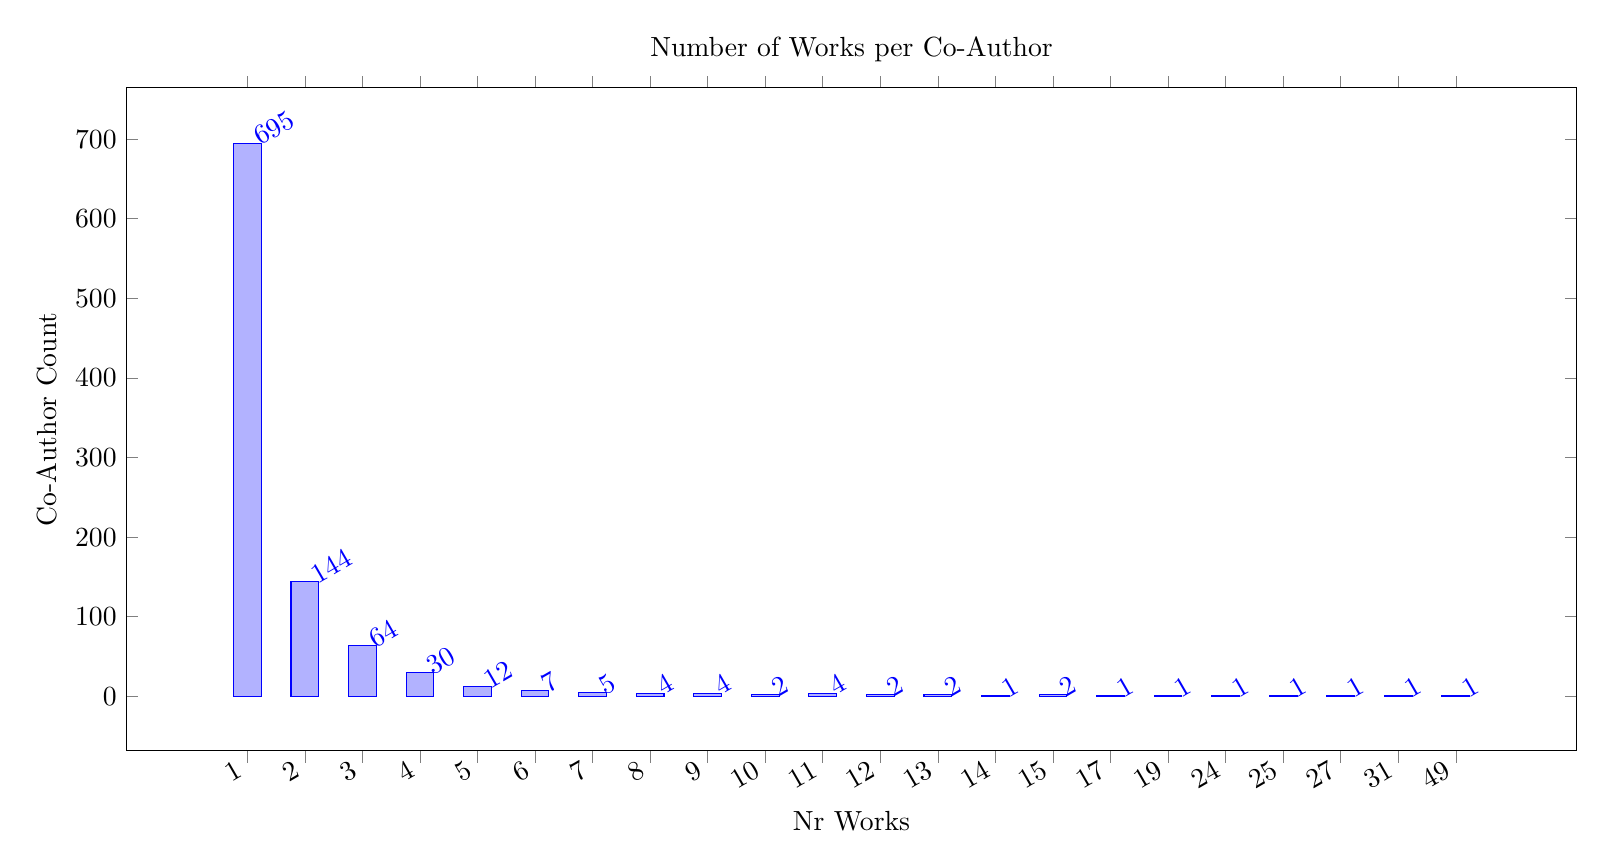
\begin{tikzpicture}
\begin{axis}[title=Number of Works per Co-Author,xlabel=Nr Works,ylabel=Co-Author Count,width=20cm,height=10cm,ybar,symbolic x coords={1,2,3,4,5,6,7,8,9,10,11,12,13,14,15,17,19,24,25,27,31,49},
    xtick=data,
    nodes near coords, 
    nodes near coords align={rotate=30,anchor=west},
    x tick label style={rotate=30,anchor=east},
]
\addplot+[] coordinates {
(1,695.000000)
(2,144.000000)
(3,64.000000)
(4,30.000000)
(5,12.000000)
(6,7.000000)
(7,5.000000)
(8,4.000000)
(9,4.000000)
(10,2.000000)
(11,4.000000)
(12,2.000000)
(13,2.000000)
(14,1.000000)
(15,2.000000)
(17,1.000000)
(19,1.000000)
(24,1.000000)
(25,1.000000)
(27,1.000000)
(31,1.000000)
(49,1.000000)
};
\end{axis}
\end{tikzpicture}

\end{document}
